\vspace{10pt}

{\centering\subsection*{邓梓欣:元宵节}}

\addcontentsline{toc}{subsection}{邓梓欣:元宵节}

\renewcommand{\leftmark}{邓梓欣:元宵节}

\begin{figure}[htbp]

\centering

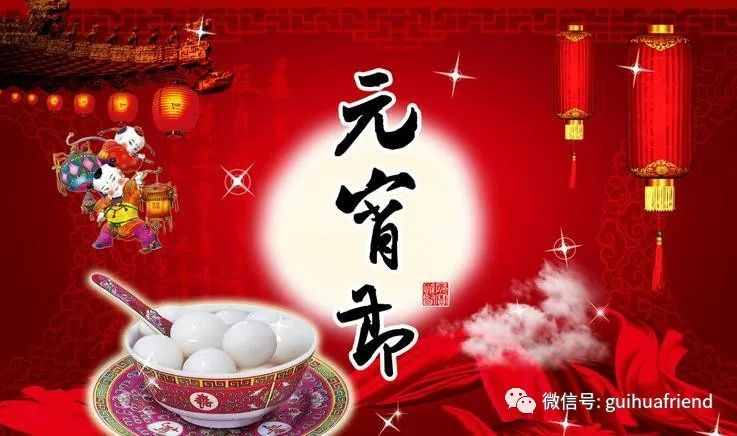
\includegraphics[width = .5\textwidth]{./ch/37.jpg}

\end{figure}



“离家十里远,别是一乡风。”我们的祖国幅员辽阔,民族众多,每个地方都有自己的风俗习惯。

我的家乡在长江以南的湖北咸宁,在这里,我最喜欢的节日就是元宵节了。

   在元宵节这天,大人们会去大街上赏花灯。孩子们则提着各式各样、明亮的花灯去街上跑跑闹闹。天上是冷冷清清的,冷清的连一颗星星也没有,地上却是一片花灯和人的海洋:房檐上挂着花灯;有名的或大一点的铺子都要挂出几十乃至上百盏的花灯;就连人们的手上都提着花灯。花灯有许多种,许多形状的:有动物灯,那动物做的栩栩如生,仿佛下一秒就要跳到你跟前似的;有玻璃的,里头是清雅的白光,但白光透过有色的或无色的玻璃,射在地上的时候就变成了一幅美丽的画了;有西瓜做的;把西瓜的一半吃空,把外面的绿色的瓜皮削掉,只剩白色瓜囊时就把蜡烛插进去,透明灯,也很有趣;甚至有的别出心裁做出了冰灯,冰灯的做法与西瓜灯相似,冰灯晶莹剔透,光透过水凝成的冰,会发出五彩的颜色,十分光彩夺目……

街上的人也很多,在赏花灯时,我仗着个子小,便“走马观花”,才过了一会儿,我和家人便被人群冲散了。我回头一望,只看见了一眼望不到边的人群,就连马路都变成了人行道。这还不够,我就像是上了一辆已经超载了十几人的公交车,几乎连一只蚂蚁都塞不进来了。不过,就算人再多,我也要出来看花灯,因为花灯真的太好看了,而且我自己也很喜欢热闹。   其实关于闹花灯,还有一个传说呢,在很久以前,一只神鸟迷路,被猎人打死了,天帝便想烧死大家,天帝之女善良,通知了人们,人们想了个主意:“在十四、十五、十六这几天夜夜灯火通明,张灯结彩。”于是人们骗过了天帝。闹花灯的习俗,也因此流传下来。   元宵节还要吃元宵,这象征着团圆甜蜜,大家在这一天还会放鞭炮呢!    元宵节是春节的句号,过完元宵,我们就要上学了,甜蜜的春节又走了……





\vspace{10pt}



作者:六(3)班 邓梓欣



指导老师:刘嘉蕾



投稿:2021年4月21日



发表:2021年4月25日






                



\vspace{10pt}

\hline



